  % hello.tex - our first latex example

\documentclass[a4paper]{report}
\usepackage{titlesec}
\usepackage{graphicx}
\usepackage{framed}
\usepackage{pdfpages}
\usepackage{wrapfig}

\addtolength{\oddsidemargin}{-.5in}
\addtolength{\evensidemargin}{-.5in}
\addtolength{\textwidth}{1in}


\title{MOS : A Multitasking Operating System}
\date{\today}
\author{Michael Rochester\\ Candidate: 23344\\ University of Sussex
        \and Supervisor:\\ Martin Berger}


\setcounter{tocdepth}{4}
\setcounter{secnumdepth}{4}
\begin{document}

\titlespacing*{\chapter}{0pt}{-50pt}{20pt}
\titleformat{\chapter}[display]{\normalfont\huge\bfseries}{\chaptertitlename\ \thechapter}{20pt}{\Huge}


\maketitle

\tableofcontents
\listoffigures

\chapter{Introduction}

The overall aim for this project is to produce a simple Multitasking Operating System (herein called MOS), following 5 key tenants, to study structure, allocation, and management of different classes of resource. This section provides a brief introduction to Operating Systems, Discusses the project aims, and looks at the approach take.

We live in a world surrounded and controlled by machines, and software is our way of telling those machines how to act. As our machines and needs become more complex, so must the software that runs them. An Operating System is a software package that allows for others to easily create complex behaviours by providing simple high level abstractions over the intricate low level hardware.

















\clearpage
\section{Understanding Operating Systems}


Before this project can even begin, an understanding of what a Operating System is and does is required.

Operating Systems come in all different shapes and sizes, however usually they contain three distinct parts:

The kernel is the software that drives the hardware. It provides nice abstractions and interfaces to control the very fiddly underlying machine.

The Bootloader is the code that is run first. It gets things that the kernel might need set up, for example, getting the CPU into the correct operation mode.

The Final part is a collection of programs and other software that come with the Operating System. Although some people would argue this is not so much part of the Operating System, on some systems (namely Microsoft's Windows) a huge number of these programs are built right in, and seem from the outside to be part of the kernel.

\subsection{The Bootloader}

\begin{figure}[ht]
\centering
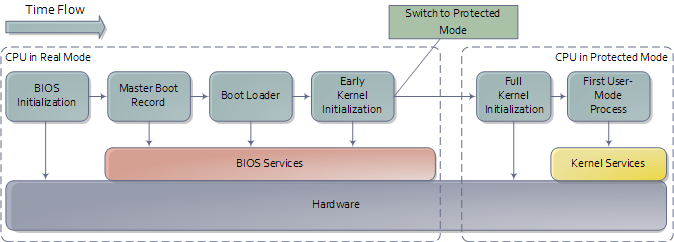
\includegraphics[width=415px]{images/bootProcess.png}
\caption{An Example of a boot cycle. The bootloader is in control while the CPU is in Real Mode.}
\label{fig:theloader}
\end{figure}

The bootloader's job is to load the kernel. First off, the CPU has to begin executing code somewhere, most of the time this is done by the BIOS, which detects our bootloader and starts it running.

The majority of the rest of the bootloader's job is to get the hardware ready for the kernel to take over. Tasks like detecting the available physical memory of a machine is up to the bootloader, once it has gathered such information, the loader will store it somewhere the kernel can find it.

The final steps of the bootloader are to get the CPU into the right mode. It does this by first setting up some important `tables' in memory. One of these tells the CPU what to do if an interrupt is produced. Another tells the CPU where it can find physical addresses in RAM when virtual addresses are looked up.

Finally the bootloader can jump to the start of the kernel and it's job is finished.

\clearpage
\subsection{The Kernel}

\begin{wrapfigure}{r}{150px}
\centering
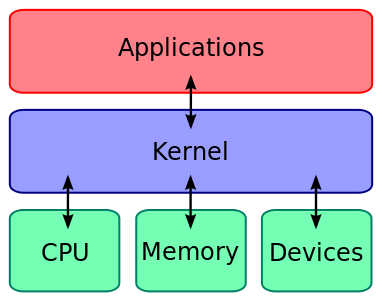
\includegraphics[width=150px]{images/kernel}
\caption{The Kernels Role is to make using the hardware easier for programs.}
\vspace{-10pt}
\label{fig:thekernel}
\end{wrapfigure}

Once the bootloader has passed control to the kernel, the kernel begins to prepare for executing programs. It will create tables of information, most of which will be empty to begin with, but they will quickly be filled. Some of the more important tasks are keeping track of which processes are currently executing and deciding which should go next, as well as ensuring that all processes think they have enough memory to operate correctly.

Once the kernel is happy that everything is in order, it will begin execution of the first process. For the rest of the time the computer is on, `processes' will be run. These processes are pieces of code that perform some form of task, each having a unique environment. As far as a process is concerned, it owns the whole computer. However, as programmers are aware that each process does not own the whole computer, they can program complex interprocess interactions, with the kernels help of course.


\subsection{The Built in Programs}

\begin{wrapfigure}{r}{250px}
\centering
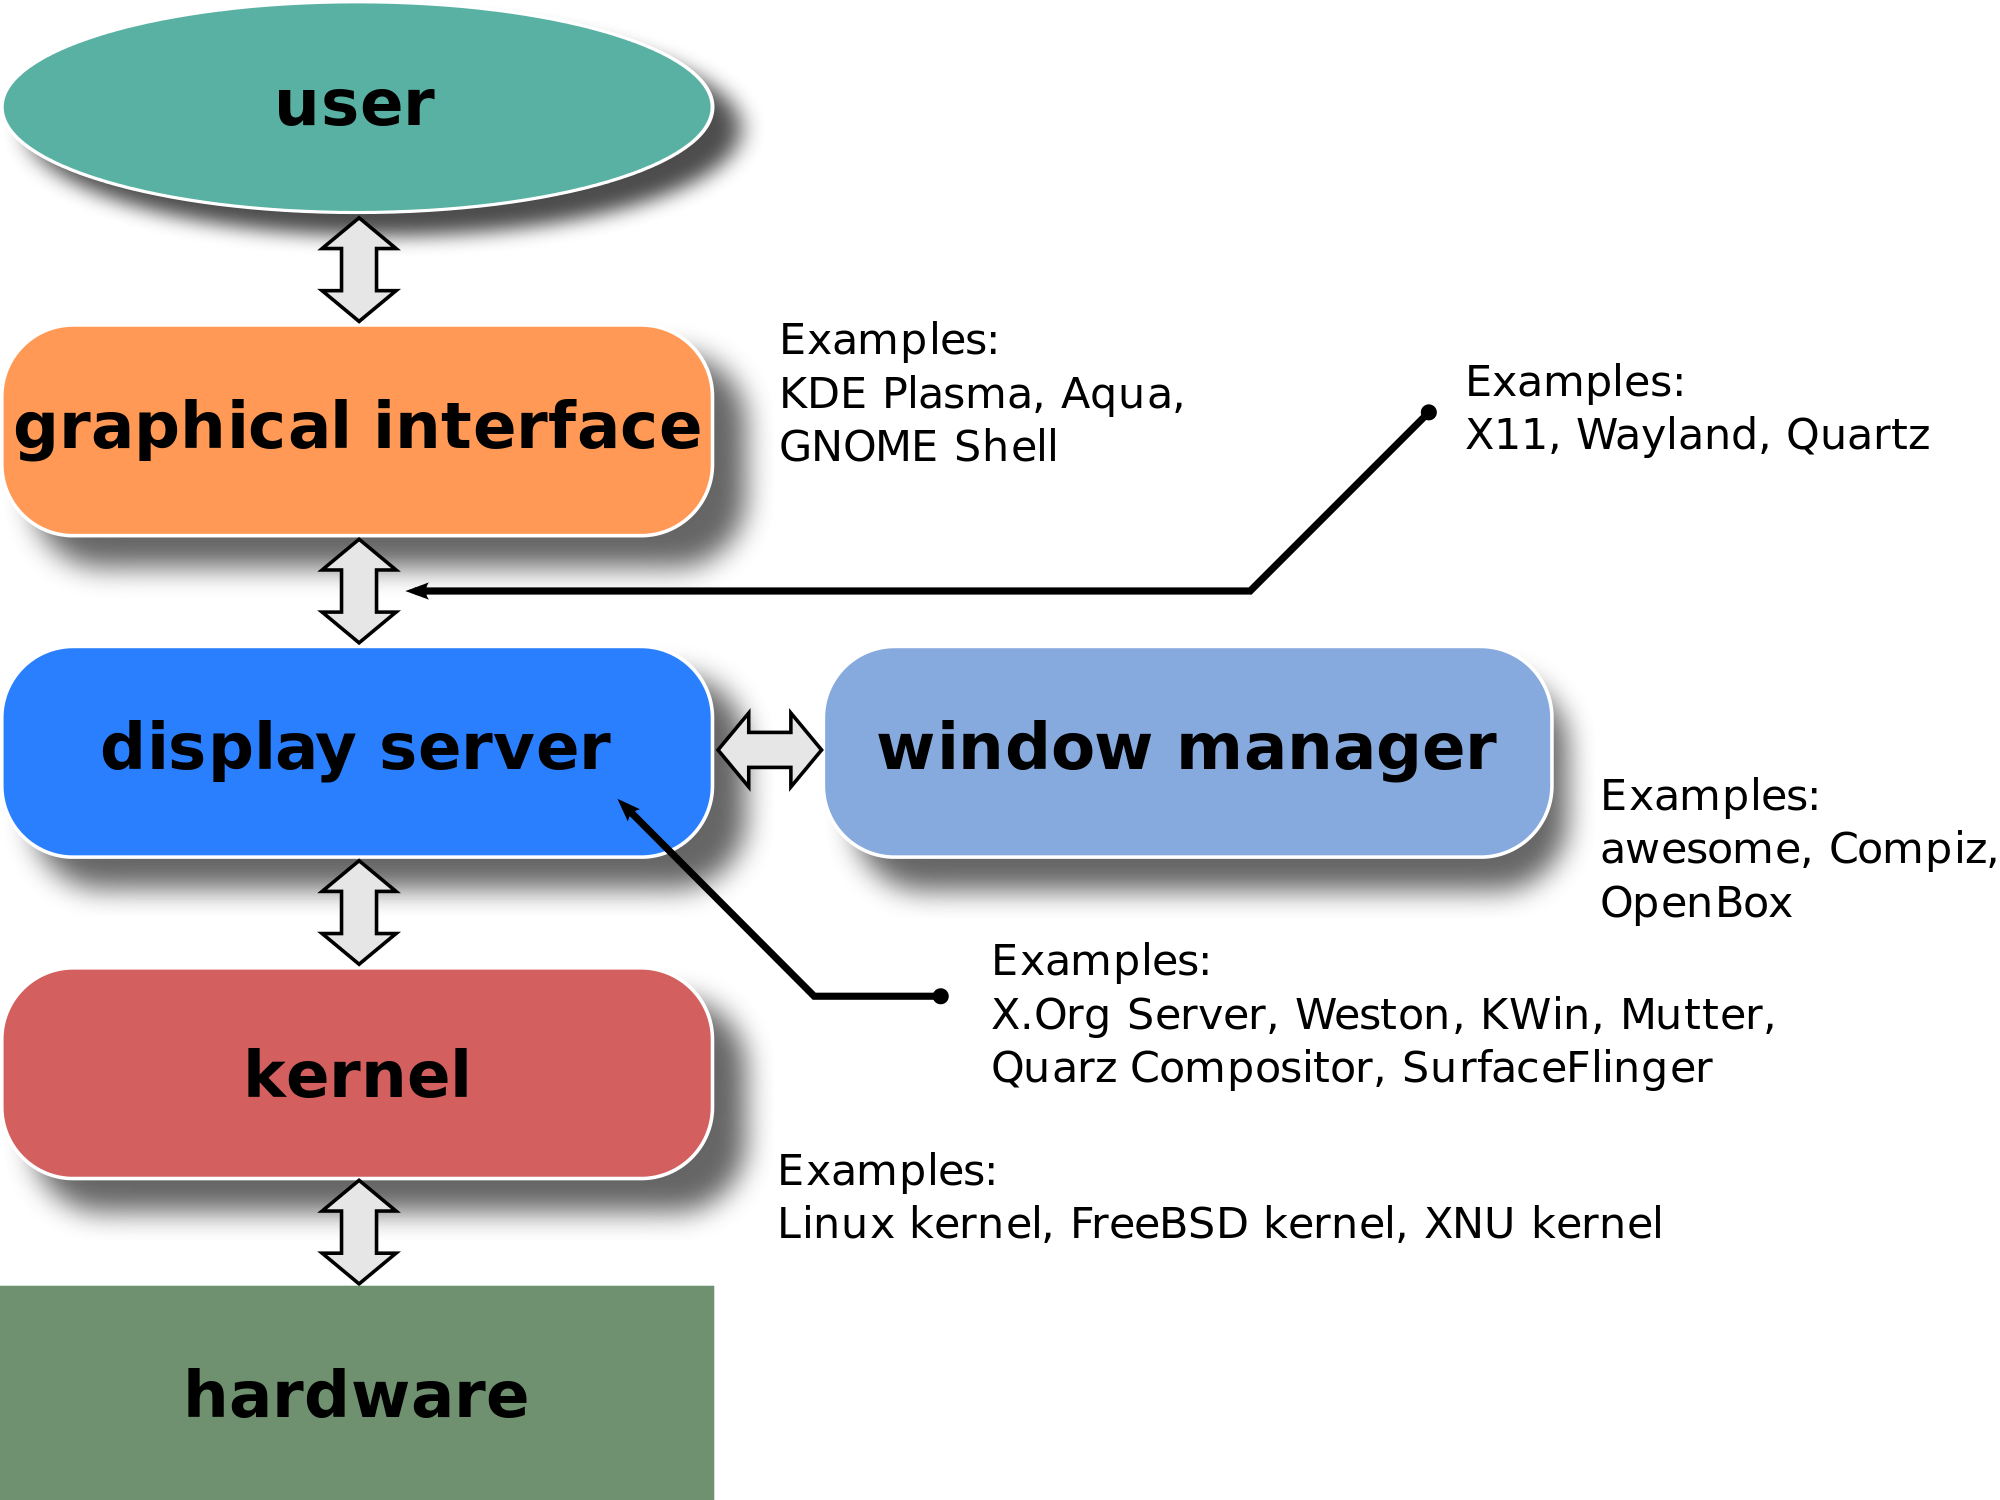
\includegraphics[width=250px]{images/windowing}
\caption{An example windowing server architecture.}
\label{fig:theserver}
\end{wrapfigure}

After the kernel starts process 0, process 0 is free to spawn many other programs. Many of these programs will come `built in' to an Operating System to create a richer platform for users.

Some would argue that these programs are not part of the Operating System its self. For example, in the Linux terminology, a kernel plus a collection of programs is referred to as a `Distro' or distribution of Linux. In Windows however, many of these programs are well integrated into the kernel and are considered part of the Operating System.

Figure \ref{fig:theserver} shows how even showing simple windows on the screen requires many levels of different programs interacting with each other. This architecture is favored amongst some computer users as it is more flexible and customizable to their own needs.
















\clearpage
\section {Project Aims}

The project was begun with a number of Primary and Extended Objectives, however as the project progressed, new objectives were discovered. These new objectives were prioritised over other extended objectives. This lead to some of the original extended objectives being left incomplete.

\textbf {Primary Objectives:}

\begin{itemize}
\item Create a bootloader to boot a kernel.
\item Create a kernel that should be able to:
\begin{itemize}
\item Load multiple `programs' into memory.
\item Execute multiple `programs' pseudo simultaneously using time sliced scheduling.
\item Allow multiple `programs' asynchronous access to areas of the terminal screen.
\item Allow for the management of the execution state of each `program'.
\item Allow each `program' access to a unique memory space.
\item Allow `programms' to asynchronously send data to each other.
\item Handle all common cpu interrupts and resolve them correctly.
\item Handle keyboard input and allow programs to `collect' keyboard inputs.
\end{itemize}
\item Create a small set of `programs' with which to test the kernel.
\end{itemize}

\textbf {Extended Objectives:}


\begin{itemize}
\item \lbrack Complete\rbrack Add some hardware drivers to load programs off disk and have some persistence.
\item \lbrack Partially Complete \rbrack Implement the entire c standard library.
\item Move into pixel graphics mode.
\item Use Multiple core's to have `true' concurrency.
\item Port the `Python' runtime to my OS (here I have chosen Python simply because there is a well documented `todo' list for porting python to new OS's).
\end{itemize}

\textbf {New Objectives:}


\begin{itemize}
\item \lbrack Complete\rbrack Create A user manual.
\item \lbrack Complete\rbrack Create A Developers manual.
\item \lbrack Complete\rbrack Create set of scripts for getting the source code, Building the project, and deploying it to a computer.
\end{itemize}















\chapter{Professional Considerations}

As this project falls within the bound of Computer Science, It will comply with the British Society of Computing (BSC) Code of Conduct \cite{CoC}. Although there is no contractual obligation to follow this code, it is important to recognize and comply with them to ensure the integrity of the project.

Each of the four main sections of the Code of Conduct will be discussed in order;

\section{Public Interest}

For this project no user information is gathered and the project poses no risk to a users health, privacy, or well-being.

The project makes use of third party material, however only within the licenses set out by those third parties that have been implicitly agreed to by all project members. Furthermore, it is explicitly marked where third party technologies were used.


\section{Professional Competence and Integrity}

The project was created as an undergraduate Final Year Project for a computer science course. It pulls knowledge from many of the modules taught as part of this course.

During the completion of the project The project engineer, Michael Rochester, will meet with a supervisor to ensure that he maintains professional competence and considers ideas and viewpoints he may not have considered.

\section{Duty to Relevant Authority}

A structure of meetings, and other feedback channels have been established between the project engineer, Michael Rochester, and the supervisors to ensure he is working in accordance with the University of Sussex guidelines.

\section{Duty to the Profession}

The project engineer, Michael Rochester, will carry out this project to the highest standard possible to maintain the reputation of the profession, furthermore all materials produced as part of this project will be freely available to any member of the profession to help further the understanding of the project domain.

\section{Requirement for ethical review}

This Project is a technical exercise in understanding the low level relationship between hardware and software, due to this, the project does not require human participation, testing, or feedback. As such, The Project does not require an ethical review, and there are no ethical concerns with this project.

\clearpage
\chapter{Requirements Analysis}

In preparation of producing an Operating System, current generation systems were studied in detail. The features and interfaces of the systems were analysed to assist in the designing of the MOS. Although It was known in advanced that MOS was not going to be complex enough to incorporate all features of the reference systems, it was important to study what current systems do, such that their most important features could be mimicked.

Modern Operating Systems are such that there are two user groups.


The End Users are the people using the Operating System and its programs to assist in achieving an assortment of tasks. To them, the Operating System provides a few simple mechanisms to interact with the system, E.G. Launching programs, closing programs, and switching between the `focused' program. Most of the inner workings of the Operating System are hidden from the end user, and they mainly interact with the `User space programs', which are not defined by the Operating System Developer.


The Program Developers use an Operating System as a platform to create the programs the End User will use. To them, the Operating System is a Resource Manager and Scheduler and provides some crucial functionality for complex behaviours like creating new processes, Allocating dynamic memory, allocating screen space to the programs, and accesing the hard drive. Many of the complexities of the Operating System (especially hardware control) are abstracted away from the Program Developers, however it is expected that they have some awareness of how the system is structured to successfully integrate with the kernel.

\clearpage
\section{The End User}
The reference systems that were studied with the End Users in mind are: The Linux distribution remix `Gnomebuntu' and the Microsoft Operating System `Windows 8'. These systems were chosen to get a spread in our sample. The systems are both popular desktop systems, however: One, (Linux) is stemmed from an open source mentality, where the source code is freely available and the system is free, and the other (Windows) is produced by a company with the aim to provide paying business, and home customers with a usable system.

The parts of the reference systems that were analysed from the end users perspective are; program launching, process management, and program interaction as these are the main sections that will be implemented in the MOS.

\subsection{Launching programs in Linux and Windows}

In both reference systems, the `windows' key is used to expose the program launching interface.

In Windows, the interface is a customizable, horizontal-scrolling, tile-based launcher. Each tile can be set to launch an application, or even launch a sub-activity of certain applications. Furthermore each Tile can give basic information of the internal state of the programs, even when the program is not properly running. (see Figure \ref{fig:WinLaunchScreen}.)


In Linux, the interface is a alphabetized list (with icons) of installed programs, sorted into pages. Pages can be navigated with vertical scrolling, or by jumping directly to a page represented by dots to the right of the screen. Linux also provides a `quick launch bar' (on the left of the screen) that can be accessed by simple pushing your cursor to the left edge of the screen. This allows for quicker launching of your favorite programs (see Figure \ref{fig:LinLaunchScreen}.)


\begin{figure}[ht]
\centering
\begin{minipage}{.5\textwidth}
  \centering
  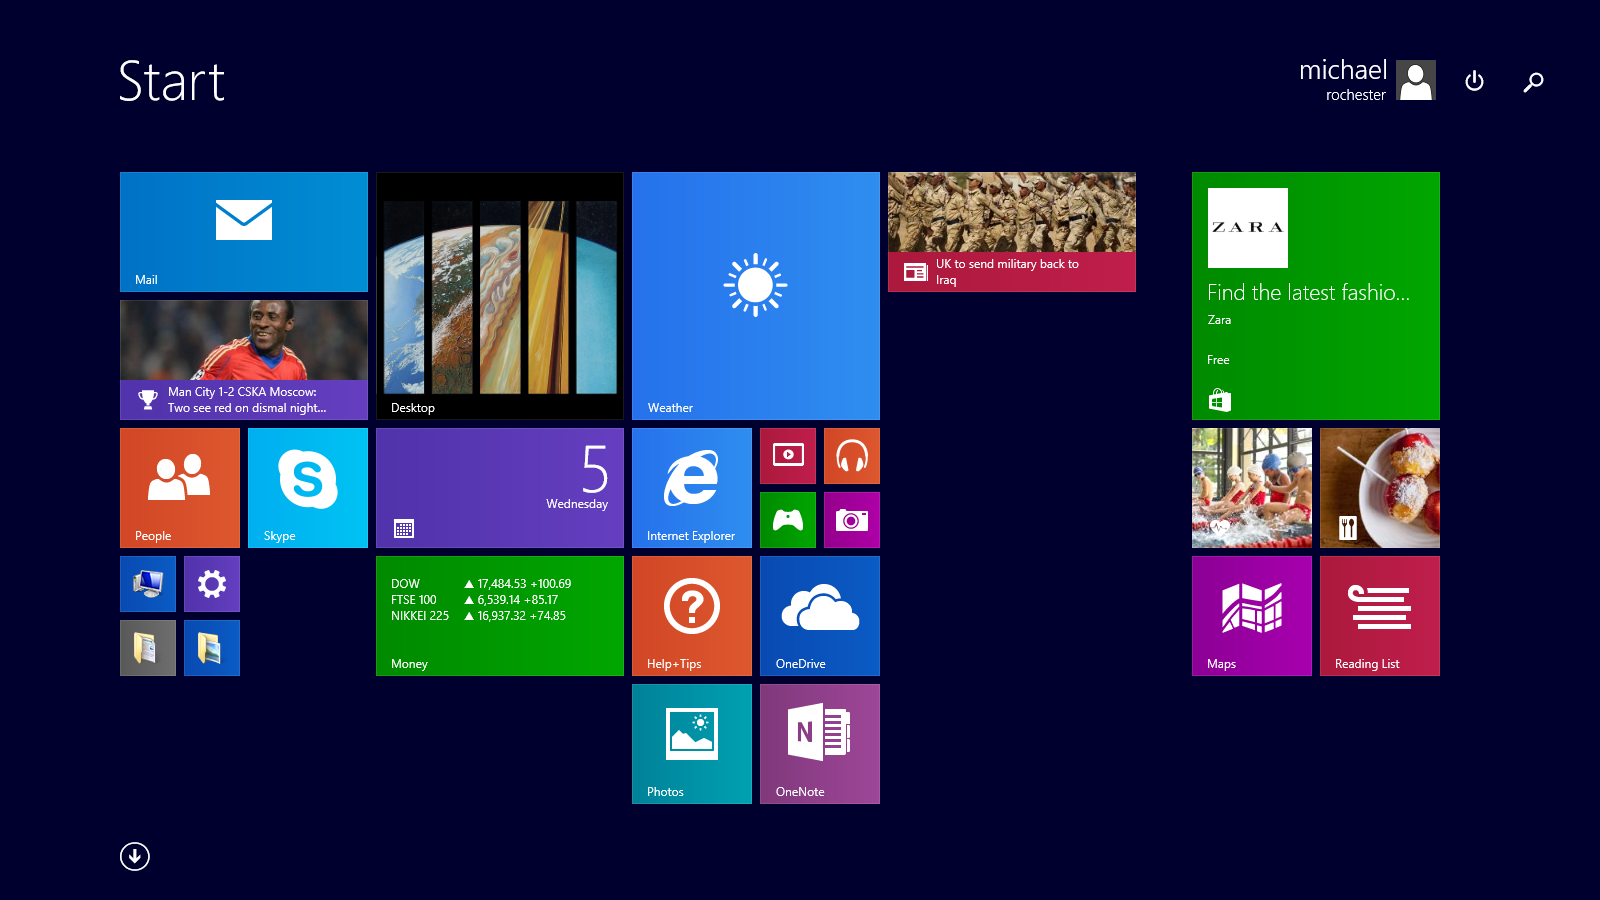
\includegraphics[width=200px]{images/Windows_Program_Launcher_Screenshot}
  \caption{Windows Program Launcher Interface}
  \label{fig:WinLaunchScreen}
\end{minipage}%
\begin{minipage}{.5\textwidth}
  \centering
  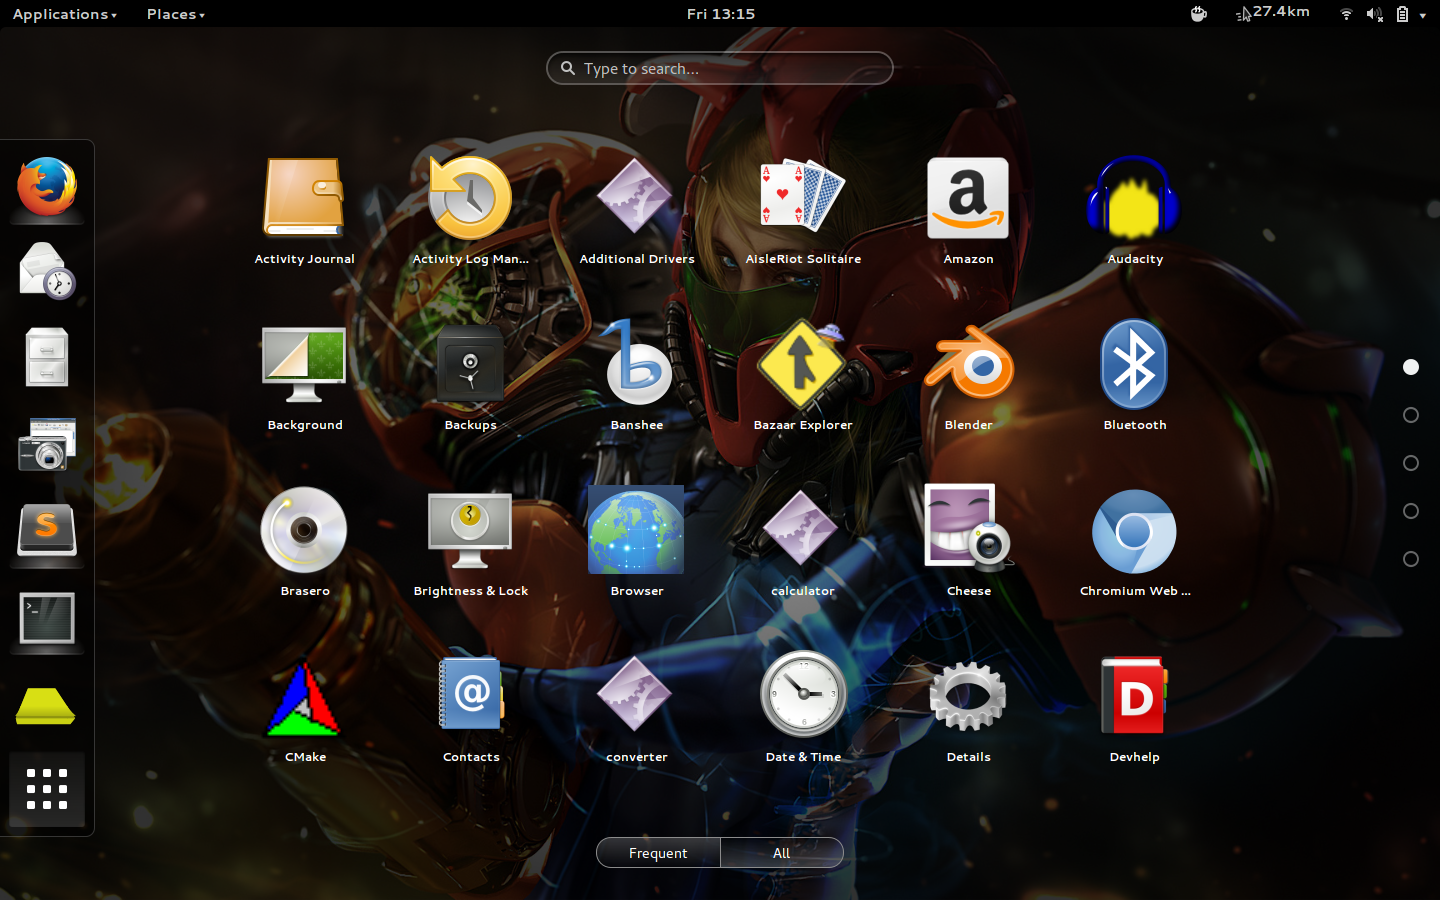
\includegraphics[width=200px]{images/Linux_Program_Launcher_Screenshot}
  \caption{Linux Program Launcher Interface}
  \label{fig:LinLaunchScreen}
\end{minipage}
\end{figure}


\subsection{Managing running programs in Linux and Windows}

Both reference systems provide a way of interacting directly with the process manager to give the user power over which programs are running on their system.

In each system, the process manager is very similar, as the tasks they perform are identical. Both systems provide a window that lists processes and some relevant information about each process like PID, cpu usage, memory usage, disk usage, and network usage. It was found that the majority of these fields are concerned with what resources a process is using. This is the case because an Operating System's purpose is to manage the physical resources available to the software.

Each system also provides the ability to change what information is provided for each process, these extra informations include many other physical resource usages (I.E. Nice value, or cpu time) as well as a more in depth view of the default informations (I.E. separating `memory usage' into: Virtual, Resident, Writeable, Shared, and Xserver memory.)

In each system this list was scrollable, allowing for many more processes that can fit in the window, furthermore the window becomes horizontally scrollable if the information exceeds the width of the screen.

Both systems provide a simple way of pausing or ending processes to manually free up resources being used by those processes.

Figures \ref{fig:WinProcManScreen} and \ref{fig:LinProcManScreen} show the process management screen in both the reference systems.

\begin{figure}[ht]
\centering
\begin{minipage}{.5\textwidth}
  \centering
  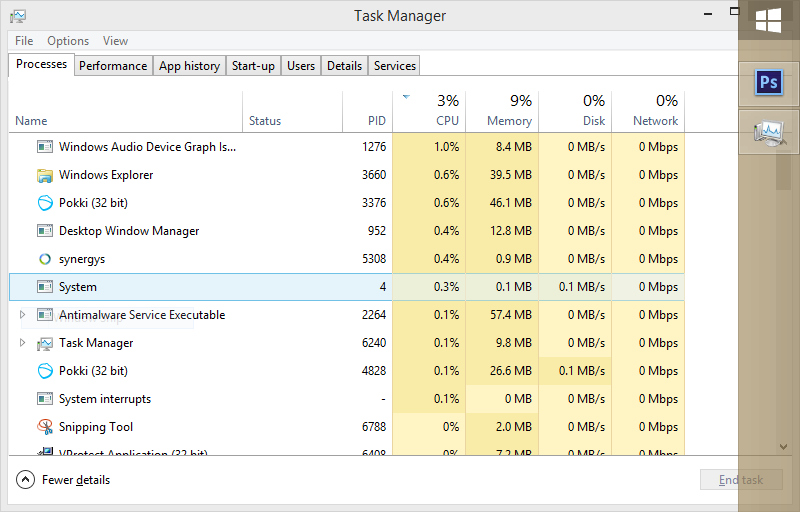
\includegraphics[width=200px]{images/Windows_Program_Manager_Screenshot}
  \caption{Windows Program Manager Interface}
  \label{fig:WinProcManScreen}
\end{minipage}%
\begin{minipage}{.5\textwidth}
  \centering
  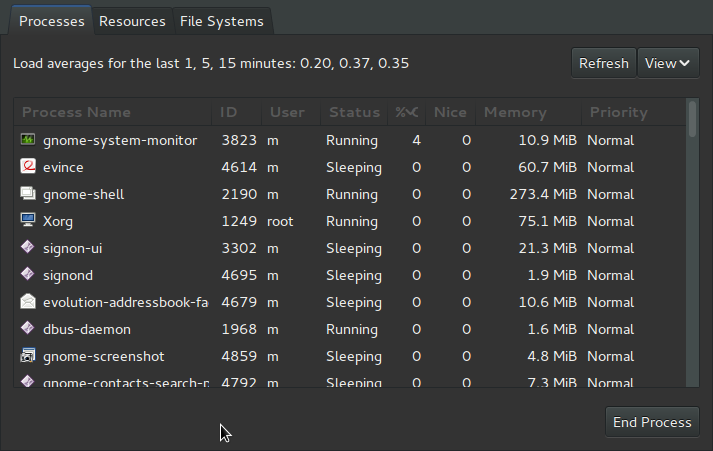
\includegraphics[width=200px]{images/Linux_Program_Manager_Screenshot}
  \caption{Linux Program Manager Interface}
  \label{fig:LinProcManScreen}
\end{minipage}
\end{figure}


\subsection{Using programs in Linux and Windows}

Interacting with programs is what users spend the majority of their time on a computer doing, because of this, it is a pivotal design aspect in modern Operating Systems. Some systems can be very different in how they allow you to interact with programs. Although the two reference systems were similar in how they present the programs to you, they differed when it came to navigating between programs.

In both the reference systems, the programs were presented in `floating', overlapping windows. These windows share the screen space by having the `active' window draw on top of all other windows. The system provides a way or moving, hiding, and resizing the windows to customize your workspace. Both systems provide similar mechanics for achieving this. They each provide a `title bar' that can be grabbed and dragged around to move the window. Each also provide the ability to grab the very edge of any side of any window, or the corners, to resize the window to the desired size. Finally, each system provides buttons to manipulate the windows more directly. This is where the systems begin to differ.

The Windows Operating System provides three buttons; The first Button allows the user to minimize the window to hide it from the work space. The second button is to maximize/un-maximize the window, this makes the window occupy the entirety of the screen. The final button exits the application.

The Linux Operating System only provides an exit button.

Figures \ref{fig:WinTitleBarScreen} and \ref{fig:LinTitleBarScreen} give example of these features.

\begin{figure}[ht]
\centering

\includegraphics[width=200px]{images/Windows_title_bar_screenshot}
\caption{Windows Title Bar Example}
\label{fig:WinTitleBarScreen}
\end{figure}

\begin{figure}[ht]
\centering

\includegraphics[width=200px]{images/Linux_title_bar_screenshot}
\caption{Linux Title Bar Example}
\label{fig:LinTitleBarScreen}
\end{figure}

Because of the nature of overlapping windows on both systems, it is possible for one window to be drawn entirely `under' another window. In Windows it is in fact possible to choose to hide a window from the workspace completely. In this situation the systems both provide different ways to navigate back to the `hidden' window.

On windows, There is a `task bar'. This is a portion of the screen, (often located at the bottom of the screen), that stores small icons for each running program. Clicking on one of these icons will bring that program to the front, un-minimize it, and make it the `active' program.

On Linux, Pressing the windows key, or pointing your mouse cursor to the corner of the screen shows you all of the open programs by `zooming out' and separating all the programs from each other. Selecting a program from this `exploded' view will un-minimize this window, bring it to the front, and make it the active window.

Figure \ref{fig:WinWinNavScreen} and \ref{fig:LinWinNavScreen} give example of these Navigation features.

\begin{figure}[ht]
\centering
\begin{minipage}{.5\textwidth}
  \centering
  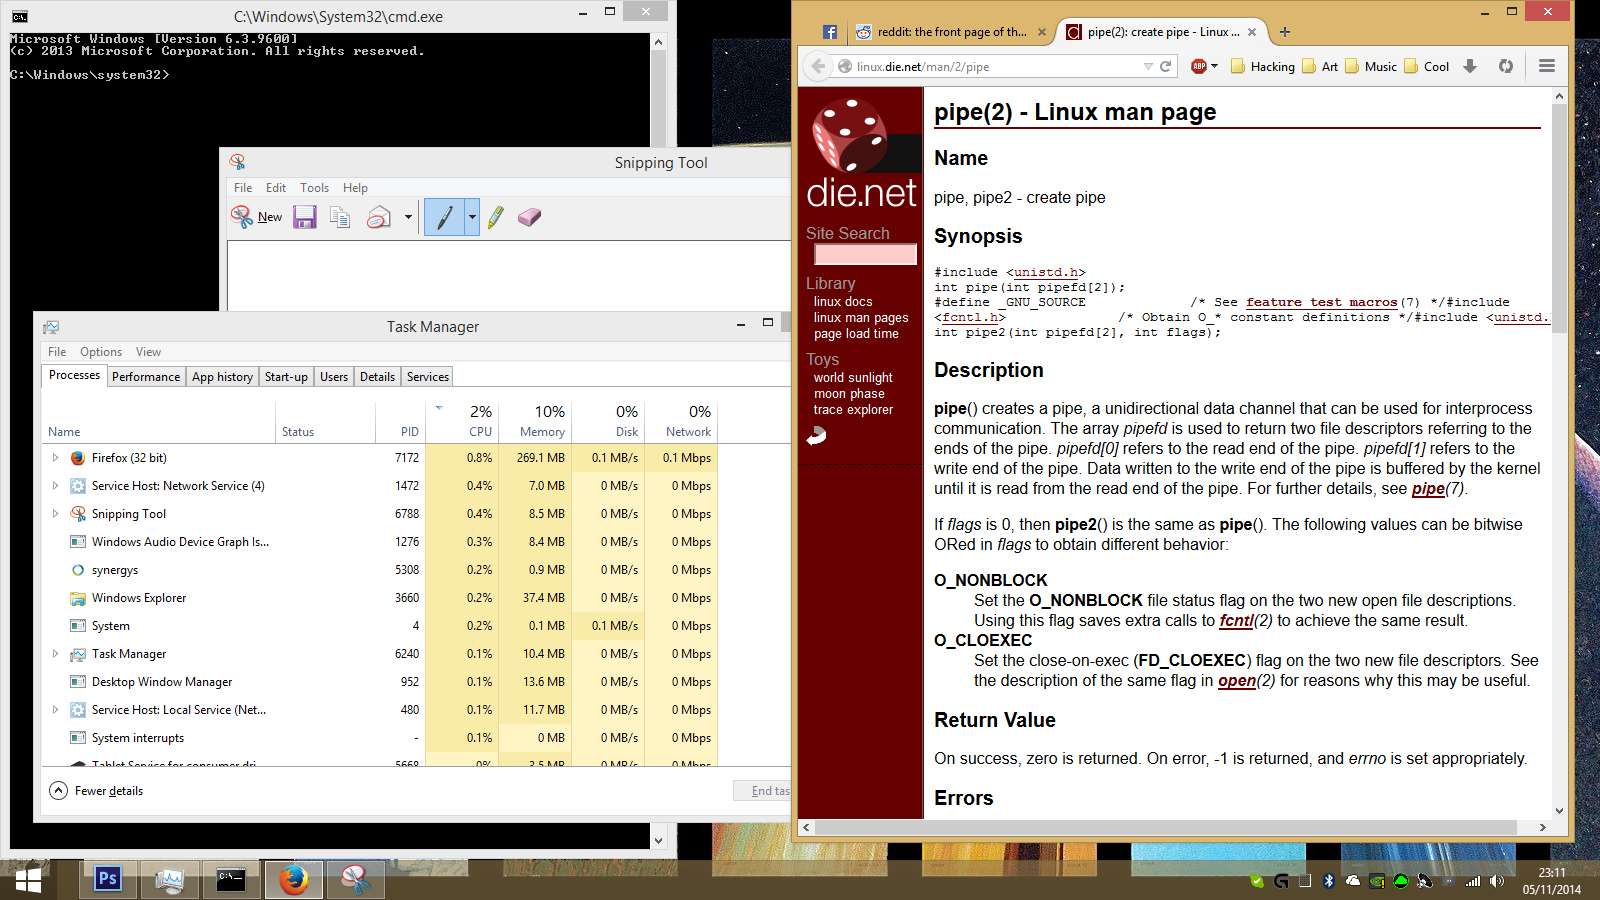
\includegraphics[width=200px]{images/Windows_Window_Navigation_Screenshot}
  \caption{Windows Program Navigation Interface}
  \label{fig:WinWinNavScreen}
\end{minipage}%
\begin{minipage}{.5\textwidth}
  \centering
  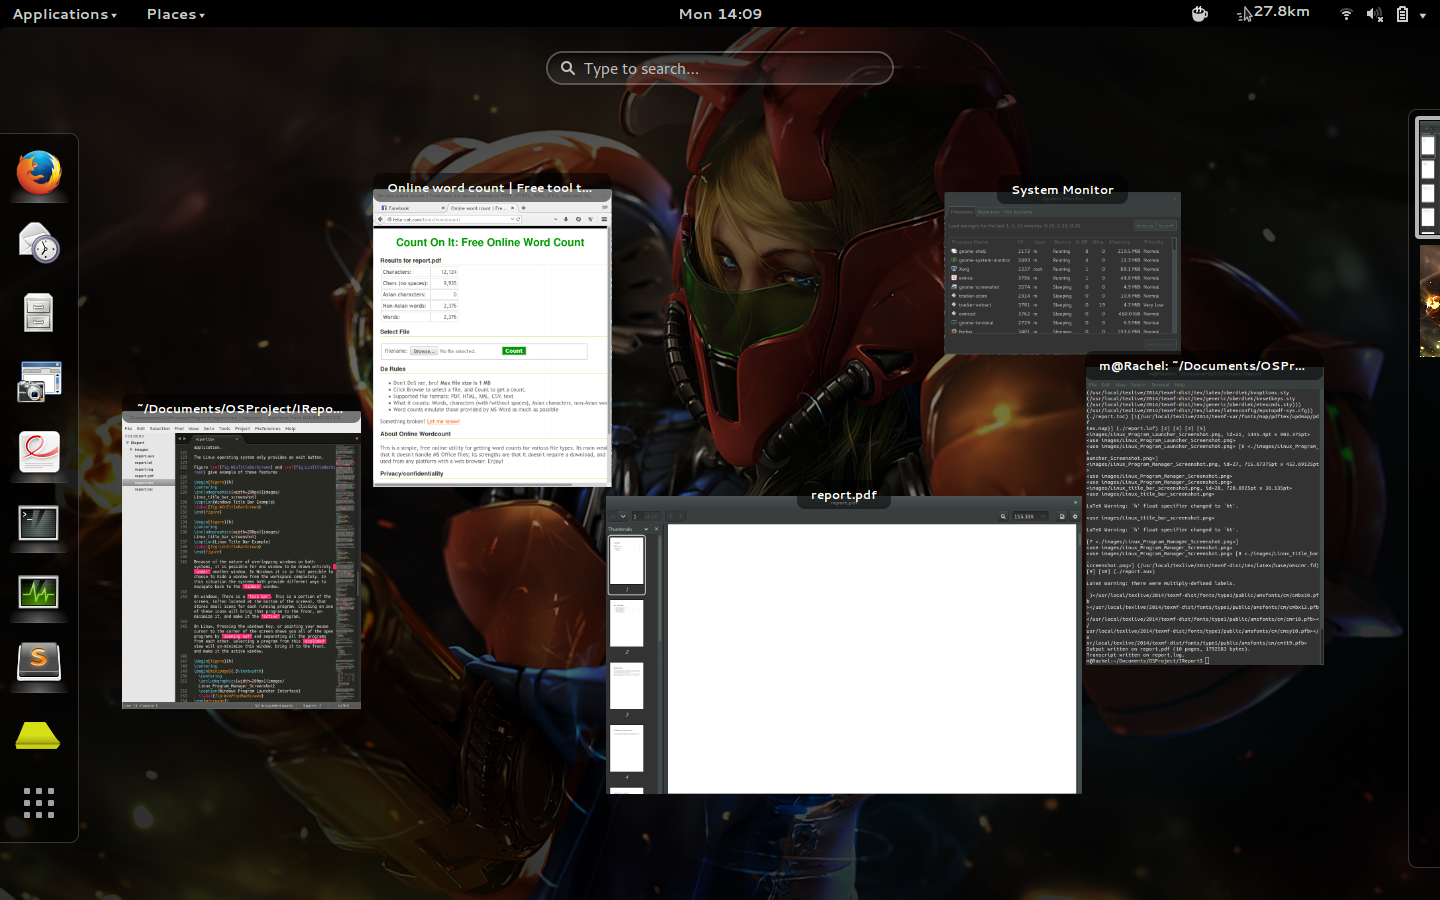
\includegraphics[width=200px]{images/Linux_Window_Navigation_Screenshot}
  \caption{Linux Program Navigation Interface}
  \label{fig:LinWinNavScreen}
\end{minipage}
\end{figure}


\clearpage
\section{The Program Developers}

To understand how program developers interact with Operating Systems The Linux distribution remix `Gnomebuntu' was studied. Only one system here was studied as Linux is an open source system. This meant that the system could be looked at in more depth.

The parts of the Linux system that were analysed are the; Process management system, the memory management system, the windowing system, and Inter Process Communication.

\subsection{Managing processes in Linux}

Linux exposes a number of system calls to the program developers to allow them to create, destroy, and pause processes, and also change the current `executable' to allow for new programs to be run.

\noindent
\textbf{Creating a new process}

To create a new process, Linux provide the `fork' system call. \cite{manFork}

Fork will spawn a new processes with a perfect copy of the calling processes memory and cpu state. This effectively means that fork will return twice, once into the caller and once into the child. It will return 0 to the child and the child pid to the parent.

\noindent
\textbf{Changing executable}

To change the executable that your process is running Linux provides execve. \cite{manExecve}

Execve will replace the calling processes memory with that of the target executable and then jump to the \_\_start label in the target executables code. This allows for switching into new executables and can be used along side fork to spawn new programs.

\noindent
\textbf{Destroying processes}

To destroy a process, Linux provides the `kill' system call. \cite{manKill}

In Linux, kill is not just for killing processes. It allows the caller to send a signal to the target process. Frequently the signal sent is SIGKILL or SIGTERM which both destroy the target processes in different ways.

\noindent
\textbf{Pausing and Restarting processes}

To pause and continue processes in Linux, the kill system call is re used, but now the caller sends the SIGSTOP signal.

\subsection{Managing memory in Linux}

Linux provides two functions for memory management, one to allocate memory and one to free it.

\noindent
\textbf{Allocating memory}

Linux provides the malloc call to allocate memory. \cite{manMalloc}

Malloc is passed the size of memory need in bytes and will return a pointer to the heap that is at least of the size requested.

\noindent
\textbf{Deallocate memory}

Linux provides the free call to deallocate memory.

Free is passed a pointer to memory that was received from malloc, it frees this memory allowing for it to be allocated during future calls to malloc.


\subsection{Managing screen space in Linux}

The screen space is not managed by the Linux kernel and so is not useful as a study for MOS.

\subsection{Inter Process Communication in Linux}

Communication between processes is an important part of creating complex behaviours in user space programs. Linux provides some simple calls to create channels of communication between processes.

\noindent
\textbf{Creating a pipe.}

Linux provides the `pipe' system call to create pipes. \cite{manPipe}

`pipe' created a one directional communication channel and provides the user a handle to this channel.

\noindent
\textbf{Reading and Writing to a pipe.}

To use this channel, Linux provides `write' and `read': \cite{manWrite} \cite{manRead}

These system calls will read and write using the pipe, allowing process to send data to each other. Note, it is by design that the pipe only transmits bytes, it is down to the user space program to define any communication protocols for transmitting more complex data.

\section{Analysis conclusion}

It was found that in end user design, many systems share similar design features. These features are very rich and operate do to a wide collection of tool, utilities, and applications The most important of these feature should be mimicked in new systems to assist new users in understanding how the the system works, However due to time constraints MOS will target much simpler versions of these features.

From the programmers perspective. The system API's or modern Operating Systems have been well thought out and have stood the test of time, however sometimes represent behaviours far more complex than that which MOS targets. The studied API's will be mimicked both to follow tried and tested ideas, and also so that program developers feel at home developing for MOS.

































\clearpage
\chapter{Design}

As with the Analysis, the Design phase was separated into End User and Program Developer sections. However here the structure of the kernel itself was also considered and planned. The designs presented here are the final designs for the system, some earlier versions can be found in XXXXX.

Design for the end user focused on similar tools, looks, and controls to existing systems; The Linux CLI was referenced for a lot of the simple command line tools as MOS' text mode graphics share a common interface to Linux terminals. MOS programs also targeted a clean workspace, avoiding unnecessary ascii drawing and focussing on delivering the service provided in a quick and clean manner.

Program Developer design was constructed with a 'many simple tools' structure. Each system call the standard library contained was made to perform one task, rather than bunching many tasks into one more complex call. This allows developers to maintain simple, intuitive control over their resources.

\clearpage
\section{The End User}

The End Users interaction directly with MOS will be limited, as the majority of their time will be spent interacting with the user space programs running on the system. Because of this, MOS will ship with a number of user space tools for managing the system

The following actions will be possible using the built in tools.
\begin{itemize}
\item Process Creation.
\item Process Management.
\item File/directory Creation.
\item File/directory Management.
\item File editing.
\end{itemize}

\subsection {Process Creations : MASH}

MASH will be MOS' built in shell. Using MASH, users can launch any other process.

MASH will support passing parameters to launched processes, and a persistent file history. It will be displayed to the user as a single line at the bottom of the screen, with a \> prompt where the user can enter their command.

Since MASH will cover Process Creation. All other actions that user can perform with build in tools are achieved through different built in programs. The user can use MASH to launch these programs passing any desired parameters.

\subsection{Process Management : processes}

The program called processes will serve as the users tool for killing processes.

The proposed design for this program is given by the following example screen.

{\ttfamily \small
  \begin{framed}
    \begin{verbatim}

      Running Programs:

        PID     | Name     | CPU Usage     | Memory Usage  | Status     |
        0       | init     |           0 % |         8 KB  | Paused     |
      > 1       | time     |           2 % |         2 KB  | Running    |
        2       | notes    |           1 % |        25 KB  | Running    |
        5       | pong     |          80 % |       102 KB  | Running    |
        12      | name     |           0 % |         1 KB  | Paused     |

     Press k to kill the current [>] process.

    \end{verbatim}
  \end{framed}
}

As shown, this tool will show the user information about each running processes and afford them the ability to kill these processes.

\subsection{File/Directory creation: mkdir and touch}

MOS will provide two programs for creating files and directories. touch will create empty files and mkdir will create directories. Both programs will operate in a similar way, taking an absolute path as their only parameter. Neither will create anything unless the parent directory of the wanted object exists, and the parameter is well formed (with a training / for directories).

\subsection{File/Directory Management: rm and mv}

For file and directory management MOS will provide two functions.

The first is rm. rm will try to delete the object at the obsolete path path passed as its only parameter. This path must be will formed and the object must exist however rm does not mind if the object is a file or directory and will delete either. If a directory is selected, all child nodes of that directory will be delete recursively.

The second is mv. mv will take two parameters, the first will be the path to an existing file system object (file or directory) and the second will be the path to an existing directory. mv will move the specified object (and all of its children in the case of a directory) into the target directory.

\subsection{File Editing: notes}

MOS' provides a simple multi-line text editor for editing text files. The program takes one parameter which is a path to the file you wish to edit. If the file does not exist notes will create it.

Notes supports common cursor key commands for navigating the cursor and saves when ctrl+s is presses.































\section{The Program Developers}

As program developers are very familiar with how to create programs for other systems, the API for the project system was designed to be very similar to that of the Linux kernel that was analysed.

\subsection{Managing processes}

MOS will provide a very similar set of system calls to Linux, however their behaviour may be simpler.

These features were considered independently of each other except for creating a new process and changing the current executable, as these calls are so commonly used together.

\textbf{Creating a new process}

Similar to Linux the process creation pattern MOS was designed to follow the `fork and exec' pattern. Therefore MOS provides two system calls:

`fork()' will return the child pid to both the parent and the child, allowing for the processes to distinguish themselves by comparing this value to the value of the `get\textunderscore pid()' system call. On failure it will return -1.

`exec(pid)' takes the integer value of the target program to be loaded. It does not return. On failure the current process will not continue.

\textbf{Destroying processes}

Unlike in Linux, where destroying, pausing, and restarting processes uses one system call, MOS will use three separate calls.

`kill(pid)' will kill the target process, freeing all its memory and removing it from the scheduler.

\textbf{Pausing and Restarting programs}

Pausing programs is important for efficiency, therefore MOS provides the following calls.

`pause()' and `pause(pid)' will pause the target process until `wake()' is called. With `pause()' the current process will be paused and immediately revoke controls to the scheduler.

`wake(pid)' will wake the target process and allow it to be scheduled again. It will NOT cause the target process to be executed next.

\subsection{Managing memory}

The memory managemnt API will be Identical to that of Linux. Therefore MOS will provide two system calls:

`malloc(size)' will allocate a memory locations of size, and return a pointer to that location.

`free(pointer)' will deallocate the memory at a pointer.

\subsection{Managing screen space}

As the Linux screen management system cannot be mimicked in the MOS, a new one entirely was invented. This lead to one system call:

`setio(px,py,wx,wy)' will attempt to allocate the portion of the screen using the starting coordinate (px,py) and the size (wx,wy). If this failed (that portion of the screen is already allocated) the call will block. Otherwise it will reserve this portion of the screen for this process.


\subsection{Inter Process Communication}

The Interprocess Communication process will be very similar to Linux's system with one key addition.

`pipe(size, \&readpipe, \&writepipe)' will set up a communication channel of the requested size. On failure it will return one of a number of errors: -1 will indicate that the pipe cannot be created due to a lack of space, -2 will indicate that the system pipe table is full. This call will fill readpipe and writepipe with descriptors that can be passed to all the other pipe calls.

Once a pipe is set up three calls will be able to interact with it:

`write(pipe, byte)' will write the byte into the pipe. On failure it will return an error message; 1 will mean the pipe is full and 2 will mean the pipe is of the wrong type (a read-pipe not a write-pipe).

`read(pipe)' will return a positive byte representing the byte at the front of the pipe, or a negative error message; -1 will mean the pipe is empty and -2 will mean the pipe is of the wrong type.

`waitToRead(pipe)' will return a positive byte representing the byte at the front of the pipe or a negative error message; -2 will mean the pipe is of the wrong type. Note, if the pipe is empty, this call will block the process until the pipe is written to.





















\clearpage
\section{The Kernel}

The kernel was split into a number of discrete modules, each performing one simple task, or over seeing the access to one peice of hardware. These modules were originally designed to be self contained, not relying on any other modules, however it was quickly realised that some modules could be brought 'closer together' to help streamline the kernel. The most notable case of this is the scheduler and the terminal manger, the scheduler contains the process entries for each running application, including the io descriptors, these io descriptors are required by the terminal to operate, therefore the scheduler allows write access to these data structures 'cross module'.

The Kernel Loader can also be seen as a kernel module however it is special in that it does its job once at boot, and then does nothing for the remainder of the computers uptime.


The kernel design was a living structure throughout the project as it was hard to predict the exact nature of each module. The following modules will be implemented to support all suggested features:

\begin{figure}[ht]
\centering
\includegraphics[width=400px]{images/Kernel_Modules}
\caption{Kernel Module Dependencies}
\label{fig:WinTitleBarScreen}
\end{figure}

%\begin{itemize}
%\item Scheduler.
%\item Program Loader.
%\item Event manager.
%\item Pager.
%\item Physical Memory Manager.
%\item Heap Manager.
%\item File System.
%\item IDE driver.
%\item Pipe manager.
%\item IO manager.
%\item Keyboard driver.
%\item Interrupts Handler.
%\end{itemize}

\subsection{The Kernel Loader}

As this module is different from the others we will discuss it first.

The Kernel Loader can actual be seen as more of a kernel in its own right. It is the code that is loaded by our Boot loader (GRUB). The loaders job is to to coreectly configure the hardware in the CPU's Real Mode and then switch over to Protected Mode for the rest of the uptime of the CPU.

It has its own smaller Physical Memory Manager, IO Manager and XXX, To assist in its task. It then maps the kernel to the correct location in memory and jumps to the kernels entry point.

Since the kernel only executes in Protected mode, it has less direct access to physical memory, therefore the kernel loader must initialise the memory map for the Physical Memory Manager module and map this memory map into a suitable Virtual memory location.

\subsection{The Scheduler}

The schedulers task will be to maintain and update all relevant information about all running processes. This means it is responsible for creating, destroying, and switching processes. It will also provide write access to parts of the process information to other modules where necessary.

The scheduler depends on the Program Loader to load new programs from the hard disk, The Event manager organise timed events such as sleeping a processes, The Pager to provide a persistent memory space, and The Heap manager to provide memory space for passing parameters to new processes.

\subsection{The Program Loader}

The program loaders job is to prepare a Program for execution; Loading the binary into memory in an appropriate manner, setting all process table fields to correct values, and ensuring all other system modules correctly reflect the execution of a new program.

The program loader depends on the File System to load programs off disk.

\subsection{The Event Manager}

The event managers job is to track timed events. It will allow for the registration of certain types of events with an event deadline. Once the deadline is passed the Event manager will perform the requested action. This module requires that its main function 'events()' be called with some frequency.

The event manager depends on the Pager to provide a persistent memory space.

\subsection{The Pager}

The pager is the core module that provides memory to the system, it controls the CPU's page tables, mapping physical memory to virtual memory. The pager is also responsible for giving out unique sections of memory to all other kernel modules. By assigning this job to the pager, the kernel memory management is centralised, making it easier to move sections of memory around during development.

The pager depends on the following Physical Memory Manager for locating unallocated physical memory.

\subsection{The Physical Memory Manager}

The physical memory manager maintains a map of the physical memory (RAM) and can provide new physical memory pages to the pager.

The Physical Memory Manager interacts directly with hardware and so has no dependencies.

\subsection{The Heap Manager}

The heap manager allows other kernel modules to use the well known malloc and free calls, providing them with small, temporary (more temporary than the memory provided by the pager) sections of memory of any size.

The heap manager depends on the Pager to provide a persistent memory space.

\subsection{The File System}

The file system will create a file/directory tree abstraction over the IDE drives present on the system. It will provide two different mechanisms for accessing its tree; one for the kernel and one for the user space programs.

The kernel functions will be to read entire files/directories into memory, or write sections of memory into files. These functions are designed for speed and elegance and the kernel always wants to load/save entire files to disk at once.

The user space abstractions are centred around giving out handles to files, and letting programs read those programs like character pipes. These abstractions focus on requiring a significantly lower memory footprint, and building input and output piece by piece.

The file system depends on the IDE Driver for reading and writing to the Hard Disks.

\subsection{The IDE Driver}

The IDE Driver will be responsible for performing reads and writes to the Hard Drives. It will also need to contain some levels of caching as hard drives are typically very slow compared to the rest of the system.

The IDE driver interacts directly with hardware and so has no dependencies.

\subsection{Pipe Manager}

The pipe manager will maintain information on any pipes that user space programs require. These pipes will also be utilised and the main IO mechanism for user space programs.

The pipe manager depends on the Pager to provide a persistent memory space.

\subsection{The IO Manager}

The IO manager will control all IO for user interaction with processes, as well as any outputting the kernel may do. It must maintain a current rendering of all running processes screen space, and deliver keyboard input to user space processes at the users command. It should also maintain different kernel space and user space windows, allowing for the user to switch between the kernel and user process view.

The IO Manager depends on the Pipe Manager for delivering and receiving IO to the user space processes, the keyboard driver for collecting key presses, The Pager to provide a persistent memory space, and the heap manager for allocating window space to processes.

\subsection{Keyboard Driver}

The keyboard Driver handles keyboard input to the system, Its main job is to correctly pass signals along to the IO manager such that they can be sent to user space processes, however it may also detect system commands (like ctrl+tab and F1) and call the respective module to perform the expected action.

The Keyboard driver interacts directly with hardware and so has no dependencies.

\subsection{The Interrupt Handler}

The interrupt handler is the module that will correctly catch and process all interrupts, this may be seen as the controller of the kernel to some extent as it is both how the kernel receives information from hardware (E.G. when a key is presses, or a hard drive finishes an operation) and the entry point from the user space into the kernel (all system calls occur through the interrupt handles.)

Because of this it depends on many of the previous modules to provide services to user space, deliver information around the kernel, and control the state of the system. Namely, The File System, IO Manager, Pipe Manager, Scheduler, Keyboard Driver, and Event Manager.













































\chapter{Project Implementation}

This section discusses the implementation of each kernel module in turn along with implementation choices and reasoning for each decision.

What won't be discussed here is implementation of the various user space programs delivered with MOS, this is because they are out of the scope of the project and although they were required to make MOS a functional system, they are not interesting from the perspective of this report.

Furthermore the user space standard library will not be discussed. This section of code is a simple user space wrapper of the system calls.

We will discuss the more complex and central modules first, and then move onto the simpler modules after.
















\clearpage

\section{The Scheduler}


\subsection{Data Structure}

\begin{figure}[ht]
  \centering

  \def\svgwidth{\columnwidth}
  \input{Process_Table_Diagram.pdf_tex}
  \caption{The Process Table Structure}
  \label{fig:schedulerscreen}
\end{figure}


The Scheduler has a number of data structures. The central structure is the Process Table. This is a fixed size array of Process Entries. Each process entry stores all information pertinent to the processes' execution (More process information like `environment variables' may be stored on the disk). The position in the table corresponds to the PID of each process.

This structure is very slow when searching for processes with specific attributes, and also contains no information about the order in which processes were created. For these reasons the Scheduler also contains a number of linked lists, each storing a list of PID's of processes that are `interesting' in some way.

The active process list contains all processes that either want CPU time, or are known to want CPU time in the future. The list is ordered in such that the process at the front is always the lest recent to have had CPU time.

Using a linked list to store the active processes makes it very fast to select a new process to run, and as the scheduler maintains a handle to both ends of the list, both getting the first item in the list and putting something at the back of the list is O(1) time.

The Decision to keep sleeping processes in this list is due to fairness of execution. The Scheduler policy is that every process will receive one time-slice on the CPU before any processes gets a second time-slice. When a process sleeps, it is making the declaration that it will want CPU time later, just not right now. If we were to leave it out of the scheduling queue until it was woken back up by the events module, and then add it to the back of the queue, it would always be waiting too long. Alternatively, if we always scheduled it immediately after it woke up, then it might get more slices than it should. The solution it to put it in the scheduler queue while still asleep. Once it is at the front, it will stay there until it gets woken up. This means that if it wakes too early, it will still have to wait until each other process has had its fair share of time before being scheduled.

The Scheduler also maintains a list for any paused processes.

Using separate lists for each of these `interesting' attributes means there is never any need to search the process table for this information. The lists (by being utilized as queue's) can also be seen to keep the order in which the process gained the specific attribute stored.

\subsection{The Process Entry}

\begin{figure}[ht]
  \centering

  \def\svgwidth{\columnwidth}
  %\input{Process_Entry_Diagram.pdf_tex}
  \caption{The Process Entry Structure}
  \label{fig:schedulerscreen}
\end{figure}

\subsubsection{The Flags}

The Flags in a process entry store boolean information:
\begin{itemize}
\item init : This process has been created, but not initialized for execution.
\item dead : This process is dead; this entry may be reused at any time.
\item skip : This process should not be scheduled for its next one time slice.
\item paused : This process is currently asleep.
\item has\_input : This process can be sent keyboard input.
\item is\_hidden : This process has a reserved portion of screen space but is currently hidden.
\item forked : This process is a forked child of another (this will get cleared if the process calls exec).
\end{itemize}

\subsubsection{The Stack Pointers}
The stack pointers are the only registers that need to be stored and restored when performing a context shift, this is because all other registers are pushed onto the stack by the interrupt handler during the time-interrupt. The stack pointers are only valid while a process is not currently having a time slice.

\subsubsection{The Memory Map}
\begin{figure}[ht]
  \centering

  \def\svgwidth{\columnwidth}
  %\input{Process_Entry_Diagram.pdf_tex}
  \caption{The Memory Map Example}
  \label{fig:schedulerscreen}
\end{figure}

The memory map stores the physical pages of memory that this process has been allocated. Most entries are direct pointers to the physical addresses of the page being used (or arrays of such addresses). However, the heap\_physical\_page is actually the physical page that stores a list of physical pages for the processes heap (see diagram above). This is due to the large memory demand that some processes have and allows for more dynamic scaling of memory allocation.


















\clearpage

\section{The IO Manager}

The IO manager manages all input and output to and from the user-space applications, All system calls that correspond to printing tot he screen or accessing keyboard input are part of this module.

The IO manager works quite closely with the scheduler as the Process Entry for each process contains an IO part, which stores all the information relevant to IO to and from he process.

The IO manager also contains thee lists (using the same process lists implementation as the scheduler does). One for all processes that can have keyboard focus (`inputable'), one for all processes that control a portion of the screen (`outputable'), and one for all the processes that should control a portion of the screen but are hidden (`hidden').

The use of this list means that when the user requests that keyboard input or terminal output be switched to a the next process, the IO manager simply has to push the currently focused processes into the back of this list, and pop the next one from the front. This means that switching the focused processes is always O(1).

\subsection{Keyboard Input}

When a user-space program wants it access keyboard input, it first creates a pipe (using the pipe system calls as discussed later) and registers this pipe with the IO Manager. This pipe descriptor is held in the IO part of the process table.

During this registration, the IO manager also adds the PID of the requesting process to its `inputable' list.

When a key is pressed and the keyboard driver decides the key press is for the user space, it passes the character to the IO manager which simply writes the character into the input pipe provided for the currently focused process. If the process is sleeping (waiting for input) the IO manager will request that the scheduler wake the process up.

\subsection{Screen Output}

The output part of the IO Manager has more to do, since it is managing a finite and very scarce resource. To consider the screen manager `fair' we say that; 
\begin{itemize}
\item Any request for a portion of the screen by a user space process must by accepted and fulfilled.
\item A portion of the screen can only be under the control of one user space processes at any one time.
\item The user should have freedom to decide which processes they can interact with at any time.
\end{itemize}

The major problem with these rules is that rule one and two don't get along/ How can we always allow user space processes to get the part of the screen they want, and also never allow overlapping processes. The solution chosen is to hide processes if they overlap with new ones.

To acquire a portion of the screen the user space processes must register with the kernel a number of things; A pipe for printing in `progressive' mode, the coordinates for the top left corner of the requested are, and a width and height for this area.

The IO manager first appends this process to its `outputable' list and populates the IO part of the respective processes table entry with the remainder of the metrics, filling the column and row potion with 0 and 0.

It then checks for any overlapping processes, these are processes that are in the `outputable' list who's screen area collides with the new request. For any overlapping processes, the IO manager first pauses that processes, giving it the is\_hidden flag. Then it uses malloc() to request a portion of the kernels heap space of the same size as the old processes screen space. It copies the current state of this screen space into the new memory and assigns the pointer into the `snapshot' section of the IO part of the process entry. It then moves the processes from the `outputable' list to the `hidden' list. Finally it wipes the screen blank.

The above process ensures that, from a processes perspective, it always has full control over a portion of the screen. This is because when it doesn't have control of that part of the screen, it is paused and cannot be executed.

When the user requests to see one of the hidden processes, the IO manager repeats the process above, but instead checking for overlapping with the process that the user want to bring to the front. Once any overlapping processes have been correctly hidden, it copies the snapshot of the requested process back to the correct area of the screen and unpauses it, moving it back to the `outputable' list.

\section{The Flat vs List interlude}

During the discussion of the scheduler and the IO manager I have mentioned the use of lists to store PID's in a number of situations. These lists are an acceleration structure over the process table its self. In the first design, the scheduler and IO manager dealt only with the process table, however as noted above this table is very slow to use for many operations, namely searching for attributes.

For example, when scheduling a new processes, the scheduler would have to do a linear search across the entire processes table, including all dead processes. This meant that the longer the system ran (and the more processes that had been run) the slower the algorithm, even if all these processes were already dead.

Secondly, when a process requested a portion of the screen, the IO manager would also have to search the entire process table to see if any other processes overlapped.

The solution was to introduce a number of single linked lists, and maintain pointers to the head and tail of these lists.

By storing the process information in lists, we could accelerate the access algorithms in many different places.

The scheduler no longer has to search the process table at all, it simply needs to pull the next process out the front of the respective list. And although the IO manager still needs to search its list, the algorithm now need only to search the number of processes that have output, not every processes that has ever been run.

But if lists are so good, why not remove the process table all together?

The answer is two fold; Data duplication and direct addressing.

Processes may find them selfs in many of the systems process lists, An active process with input and output is in at least 3 lists at any time. If these lists directly contained the process entries, they would have to be copied many times around the system, which would make keeping them up to date slow and difficult. By having the process entries in one place and linking them into the lists indirectly, we can prevent duplication and maintain nice centralization of information.

Secondly, we often want to perform an action knowing the PID in advance; like setting a process flag of updating the IO part of a process. By storing the Process Entries in an array indexed by PID. These actions are always constant time.

Below is an over view of the the kind of accelerations using lists affords.

n is the total number of processes run for the entire uptime of the system
p is the number of active processes
o is the number of outputable processes
i is the number of inputable processes

it always holds that:
o <= p
i <= p
p <= n

\begin{figure}[ht]
  \centering

  \def\svgwidth{\columnwidth}
  %\input{Process_Entry_Diagram.pdf_tex}
  \caption{Runtime speed-ups of flat vs list.}
  \label{fig:schedulerscreen}
\end{figure}


















\section{The Hard Drive: Drivers and File systems}

\subsection{The IDE Driver}

The hardware access portion of the IDE driver was not created as part of this project as indicated in the code, It was simply simply adapted it to fit into MOS.

however caching was added above the driver to massively increases read write speeds.

The caching was necessary because hard drives are slow. But also the manner in which they are accessed is not ideal. In an IDE device, the only way of getting data on or off the disk is in 512 byte segments. This means if we want to write one byte, we must read 512 bytes into memory, change the target byte, then write all 512 bytes back to the disk. This is very slow. Especially as it is common to want to write sequential bytes to disk; writing 512 bytes would require 512 reads of disk, then 512 writes to and from the same section of the disk.

\subsubsection{Data Structure}

\begin{figure}[ht]
  \centering

  \def\svgwidth{\columnwidth}
  \input{Process_Table_Diagram.pdf_tex}
  \caption{The Process Table Structure}
  \label{fig:schedulerscreen}
\end{figure}

The primary structure here is the cache table, as above, it consists of a number of descriptors and a corresponding number of 512 sections of memory.

The caching layer provides the functions request_read and request_write.

When these functions are called, the cache first searches the cached blocks for a block corresponding to the requested read/write address. If a cache is found, the pointer to this block is returned. If there is no cache for the requested address, the data is off the disk into a new cache block.

If there are no new blocks available, the cache writes all modifies blocks back to disk, wipes the entire cache and then tries again.

It may seem inefficient to wipe the entire cache every time the cache fills, however the cache is very small, and purging it in the worst case only takes as long as writing the blocks back to disk. It is also very common for a file to be read/written (and therefore be moved into the cache) only once in the entire life of the system, so often many of the blocks we are `throwing away' wont be needed again. Furthermore the potential algorithm for a more sophisticated swap of old blocks (perhaps a working set clock algorithm) can take more time to execute every time we need one more block than simply throwing away the whole cache. Finally, at every system context shift (every 10 ms) the cache is written and purged anyway so filling the cache in that time is very rare.

This 10ms purge happens to both ensure any changes a user space processes has made to the disk is actually written and is not sat in a cache, but also because it is assumed that the next user space processes will want to access different portions of the disk and will therefore want a clean cache.

This cache is extremely efficient and reduces the number of read/writes and therefore the time its takes to read files by a huge factor, however there is still one slight slowdown, and as the hard drive is a systems biggest bottleneck, it was seen as appropriate to address it.

It is very common for the same block to be requested repeatedly, this is due to the nature of the file system discussed below. Most the file system structures are sequential bytes, and the data its self is in sequential 4096 byte sections. This means that its very common for one 512 byte hard drive block to be read/written for every byte (512 times) before we are done with it. This is only interesting because whenever a read/write is requested from the cache, it searches the entire cache table the appropriate block.

This search is slow. Especially as the block we need is almost always (511 out of 512 times) simple `the same one we used last time'. Because of this, the search algorithm remembers which block it served last request, and always checks that block first. That means that 511 out of 512 times the algorithm is O(1) instead of O(n), and the other 1 out of 512 time, its O(n+1) instead of O(n).


























\subsection{File System}

The file system used (called MRFS from here on out) was a modification of a piece of second year coursework. This coursework required the creation of a file system along with a set of file read write interfaces. These parts will therefore only be discussed briefly. A new set of abstractions were created from scratch for the user space system and these abstractions will be discussed in more detail.

These new abstractions were created due to the unsuitability of the old abstractions for user space. The old abstractions will be referred to as the kernel abstractions as they are used throughout the kernel. These kernel abstractions are unsuitable for user-space as they involve calling malloc (to request kernel heap memory), and returning a pointer to this memory. Its forbidden to return a kernel pointer into user space, and having the kernel allocate memory from the user-space heap is not very good practice. Therefore a new set of abstractions that provide handles to the file and allow pipe-like read write mechanisms were create, these will be referred to as the user-space abstractions.

Although MRFS was taken from a previously complete project, it was significantly modified #TODO

\subsection{File Directory Structure}

\begin{figure}[ht]
  \centering

  \def\svgwidth{\columnwidth}
  %\input{Process_Entry_Diagram.pdf_tex}
  \caption{Runtime speed-ups of flat vs list.}
  \label{fig:schedulerscreen}
\end{figure}

MRFS uses an inode structure, this means that every object on the disk is represented and described by an inode. Each inode can be either a directory or file. Directory have other file system objects as children whereas files have data blocks as children. Inode structures are very common structures and were therefore easy to find information on and implement. MRFS' implementation uses bitmaps for storing which inodes and data blocks have been allocated on the disk. It contains no caching as caching was done on a lower level (see IDE driver above). Every inode must be a child of another inode except for the root inode, called root or `/'. All inodes also must have names, unique to their parent node. This means that any file system object may be referenced by its name along with its inode number.

\subsection{File Directory Kernel Abstractions}

The kernel abstractions are simple in nature, most take a directory path and a file name, and operate upon that file. Those that operate on directories still take 2 strings, one as the path to the parent directory and one as the name of the directory wanted.

These abstractions all work `all at once' meaning that they deal with files as a whole; reading a whole file into memory, writing a section of memory as an entire file. This is method is fit for the kernel as it never needs to read/write sections of files off disk.

\subsection{File Directory User Space abstractions}

These abstractions are the endpoints for all file/directory system calls. The follow the open, read, close pattern, except that there is no need to close a file. To open a file or directory, the full absolute path to the object is required. The file system then returns a structure describing the file; its Inode number, its size, its names size, and two pointers, one into its data and one into its name. This structure is the same for both directories and files. The pointers into the data are initialized to point to the end of the file or directory.

Once a user-space program has acquired this structure it is used with all the remaining calls. These calls all work on a `one at a time' method. Meaning that writing or reading from a file must be done one character at a time. Reading from a directory returns one file structure at a time, where each is a valid file handle to one of the children of the directory.

These abstractions mean that storing this information and any mallocing must be done at the user-space applications discretion. It also allows for easily reading parts of a file, and updating the file without destroying all the old contents.




















\section{Pager}

The pager has no central data structure, however it does maintain a list of constants, each being the virtual memory address assigned to a specific kernel subsystem.

The pager will return these addresses upon request. Each kernel module that requires memory must go through the Pager to acquire its base address. This means that if we want to move the memory of a kernel module it would be as simple as changing one constant. This makes the modularity of the kernel much stronger as it means that no two modules can ever accidentally think they own the same memory space.

Other than the memory addresses, the pager is also responsible for paging physical memory in and out. However, it explicitly does not manage either physical memory, or keep track of which virtual pages are currently mapped (which is the job of the Physical Memory Manager, and the module that owns that virtual memory space respectively). It simply allows other modules to map/unmap/copy physical memory to virtual memory at any time.













\section{Heap manager}

\subsection{Data Structure}

\begin{figure}[ht]
  \centering

  \def\svgwidth{\columnwidth}
  %\input{Process_Entry_Diagram.pdf_tex}
  \caption{Runtime speed-ups of flat vs list.}
  \label{fig:schedulerscreen}
\end{figure}

The Heap manager uses a linked list implementation of memory management. Instead of having its own memory space for this linked list, it put it inside the kernel heap space itself. This means that each section of allocated memory has a memory header (as described above) immediately preceding it.

One issue with having this `in memory' structure is that its possible to accidentally overwrite the memory headers by writing outside the size of memory you requested. To detect this, the structure is padded with some magic numbers, these magic numbers are checked whenever the kernel frees memory and if there is a corruption it causes a system halt.

Although this might seem like an easy attack into the system; easily causing a system halt, it is not the case since this memory is accessible only by the kernel its self. Extensive testing of the kernels interaction with this module is used to ensure that the kernel never writes out side of memory bounds.

When the kernel requests a portion of memory, the memory manager simply follows the linked list from start to finish, looking for a space that is at least as large as the requested space. Once found, makes the node found not-free, and if the space is larger than the requested space, puts a new node between this node and the next node, marked to free.

If there are no nodes available, the Heap manager will request extra memory from the Pager and then retry.

when freeing a node, the Heap manager sets the node to free, but must check the node immediately preceding and following the newly freed one. If either nodes are also free, the nodes will be merged into one larger node. This ensures that each free section of memory is not split into many smaller nodes meaning that its more likely the manager can find blocks of memory of larger sizes. It also means that if all the memory were freed, the structure would be identical to the initial state.
















\section{Pipe Manager}

\subsection{Data Structure}

\begin{figure}[ht]
  \centering

  \def\svgwidth{\columnwidth}
  %\input{Process_Entry_Diagram.pdf_tex}
  \caption{Runtime speed-ups of flat vs list.}
  \label{fig:schedulerscreen}
\end{figure}


The Pipe manager has one central data structure, the pipe table. The pipe table keeps track of all registered pipes on the system, This table has three fields per entry (as shown above); the PID is the id of the process that owns the pipe, this is needed since the pipe stays in user space memory and knowing which processes it belongs to allows us to locate the correct piece of memory to read and write into the pipe. The location is the memory address of the beginning of the pipe. The mode is whether or not the pipe is a read pipe or a write pipe.

when pipe\_create is called, it gets passed a location for 256 bytes of continuous memory. This memory is the actual pipe its self. It creates two new records in the pipe table, one for reading and one for writing, the index of these two entries are the pipe handles that are returned to the calling process. 

The pipe its self is then initialized. The First 4 bytes are the read pointer, and point to the next byte to be read in the pipe body. The next 4 bytes are the write pointer, that points to the next free byte in the pipe. The rest is the body of the pipe. (this structure is shown above). 

The pipe uses a pointer chase method to allow for a seemingly continuous stream of data. This involves the write pointer progressing along the pipe body until it reaches the top, it then simply wraps to the bottom and continues progressing. In tandem, the read pointer also progresses along until the top, wrapping in a similar fashion.

If the write pointer ever reaches the read pointer, the pipe is full, and no more writes will be accepted. The call does not block, but returns an error code such that the calling processes can retry the write later.

If the read pointer ever reaches the write pointer, the pipe is empty, subsequent calls to read will return the EOF value to indicate to the calling processes that the pipe is empty.

A major issue with the implementation of this system is what to do if the owner of the pipe is not the current process. In this case, the pipe will actually not be in the virtual memory space at all (due to the memory protection mechanisms that `page out' all process memory when it is scheduled out.)

In this situation, the pipe manager will page in the required memory to a special area of the kernel space. It must page two consecutive pages in just in case the pipe crosses the page boundary.

Because this special area does not have the same base memory address as the process space, the location field of the pipe table needs to be recalculated. once this is done the read/write can be performed normally. Finally the special memory space is cleared.











\section{Interrupts handler}

The Interrupts handler has no core data structures.

The interrupts handler is the entry point into the kernel for any hardware or software interrupts.

Each interrupt is handled differently however the procedure is always the same;

\begin{itemize}

\item First all CPU state registers are pushed onto the current stack and all other interrupts are blocked.

\item Then the interrupter handler prepares any input for use, this input may be from user-space system calls, or values from hardware interrupts.

\item Next the handler performs the desired action, as each system call is handled differently this is as simply as calling the correct function in the correct module to perform the desired task.

\item The handler then prepares any output, this is usually to return values to the user space after a system call.

\item Then the handler sends a message to the interrupt chip on the mother board that the interrupt has been handled.

\item Finally the CPU state registers are popped off the stack and all interrupts are unblocked to restore the system to the pre-interrupt state.

\end{itemize}

This procedure ensures a number of things; First off, the kernel cannot be interrupted if it is inside a system call. This is particularly useful as none of the kernel module are reentrant. Secondly nothing the user space process does can effect the kernel space execution, as the entire CPU state is pushed each time. This also works in reverse meaning that nothing the kernel does can accidentally effect how the process acts. This means that from the user space processes perspective, the interrupt never took place.

















\section{Program Loader}

The program loader has no core data structures and can be seen as a sub module of the scheduler. When called it initializes the process entry for the selected processes, loads an ELF-Binary of the disk into memory, maps that memory to virtual addresses, storing these addresses in the process entry, and finally returns the entry point for that binary for the scheduler to jump to.
















\chapter{Log}


\section{Week 1}
\begin{itemize}
\item Created basic design docs.
\item Rewrite existing code to be suitable for this project.
\end{itemize}

\section{Week 2}
\begin{itemize}
\item Detect Upper Memory.
\item Test Stack Jumping.
\item Simple page frame allocator.
\item Bound all interrupts to stubs.
\item Created simple kernel threading.
\item Created a `printf' like utility.
\item Supervisor Meeting 1: This week we discussed the state of the project, some goals to hit in the upcoming weeks and the proposal report due in next week.
\end{itemize}

\section{Week 3}
\begin{itemize}
\item Implemented Paging.
\item Moved to a higher half kernel.
\item Loaded my first `user space' program.
\item Supervisor Meeting 2: This week we discussed how process creation was handled in linux and other Operating Systems, and how to move forward with concurrency.
\end{itemize}

\section{Week 4}
\begin{itemize}
\item implemented fork system call.
\item implemented exec system call.
\item Supervisor Meeting 3: This week we discussed how IPC was handled on many different system and how I could think about going ahead with IPC.
\end{itemize}

\section{Week 5}
\begin{itemize}
\item major bug fixing.
\end{itemize}

\section{Week 6}
\begin{itemize}
\item created proposal for IPC.
\item implemented IPC.
\item began work on interim report.
\item Supervisor Meeting 4: This week we discussed how to continue work on IPC and the next steps of using the IPC to abstract general process I/O.
\end{itemize}

\section{Week 7}
\begin{itemize}
\item finished work on interim report.
\end{itemize}

\section{Week 8}
\begin{itemize}
\item Study.
\end{itemize}

\section{Week 9}
\begin{itemize}
\item Sleep and Pause System calls.
\item Began implementation of IO over pipes.
\end{itemize}

\section{Week 10}
\begin{itemize}
\item Completed basic keyboard support
\item Created first iteration of Notes application.
\end{itemize}

\section{Week 11}
\begin{itemize}
\item Added input switching.
\item Added input indication: Input process now changes color.
\end{itemize}

\section{Week 12}
\begin{itemize}
\item Added hard drive support.
\item Added some file support in user space.

\end{itemize}

\section{Week 13}
\begin{itemize}
\item Created tool for writing the virtual hard drive from outside the emulator.
\item Init program now loads from disk.
\end{itemize}

\section{Week 14}
\begin{itemize}
\item Created launcher program.
\item Created process viewer program.
\item Fixed a number of MRFS issues.
\end{itemize}

\section{Week 15}
\begin{itemize}
\item Created kill system call.
\item Created Created new file abstractions.
\item Created Created testing framework and added tests for the memory manager and the file system.
\item Fixed many kernel memory leaks.
\item Added parameter passing to new processes.
\item Added PATH and cwd environment variables.
\item Added Ctrl+Tab to switch between hidden processes.
\end{itemize}

\section{Week 16}
\begin{itemize}
\item Scheduler now reuses old PID's
\item Created much better notes program with multi line editing capabilities.
\item Added cpu time metric for all processes.
\item Created `ls' and `less' programs
\item Improved processes program.
\item Added better testing for memory manager and file sytem.
\item Fixed many misc bugs.
\end{itemize}

\section{Week 17}
\begin{itemize}
\item Fixed refresh rate issue.
\item Moved time services into the kernel.
\item Create `pong'.
\item Improved file abstractions and extended them; removed all old abstractions.
\item Created `rm', `mkdir', and `touch'.
\end{itemize}

\section{Week 18}
\begin{itemize}
\item Created tests for new MRFS abstractions.
\item Added /proc/ directory for storing process state.
\item Fixed some memory violations for corner cases in MRFS.
\item Added better test tracking for high volume of tests.
\end{itemize}

\section{Week 19}
\begin{itemize}
\item Modified pong and processes to take command line parameters to define their location on screen.
\item Created Poster for poster presentation.
\item Added `man' program.
\item Allowed user-space applications to get more memory in their heap.
\item Create `fork\_bomb' program.
\end{itemize}

\section{Week 20}
\begin{itemize}
\item Moved from dual disk setup to single disk.
\item Reduced O() complexity of many MRFS calls.
\item Correctly deallocate memory when process ends.
\item MOS now boots on hardware.
\item Added command history into MASH.
\item Protected against killing shell process.
\item Created user manuals.
\item Created Developer docs.
\item Bound remainder of CPU interupts.
\item Improved Processes program/
\item Fixed many bugs with fork cycle and mrfs edge cases.
\end{itemize}

\section{Week 21}
\begin{itemize}
\item Began Final Report work.
\item Change color to black on white.
\item Fixed a number of user space bogs after doing extensive testing.
\item Localized entire project (removed absolute paths).
\item Added caching to processes program
\end{itemize}

\section{Week 22}
\begin{itemize}
\item Code Refactor.
\end{itemize}

\section{Week 23}
\begin{itemize}
\item Report work.
\item Added wait\_to\_read system call.
\end{itemize}

\chapter{Appendices}

The following Three pages are a copy of the Project Proposal document.

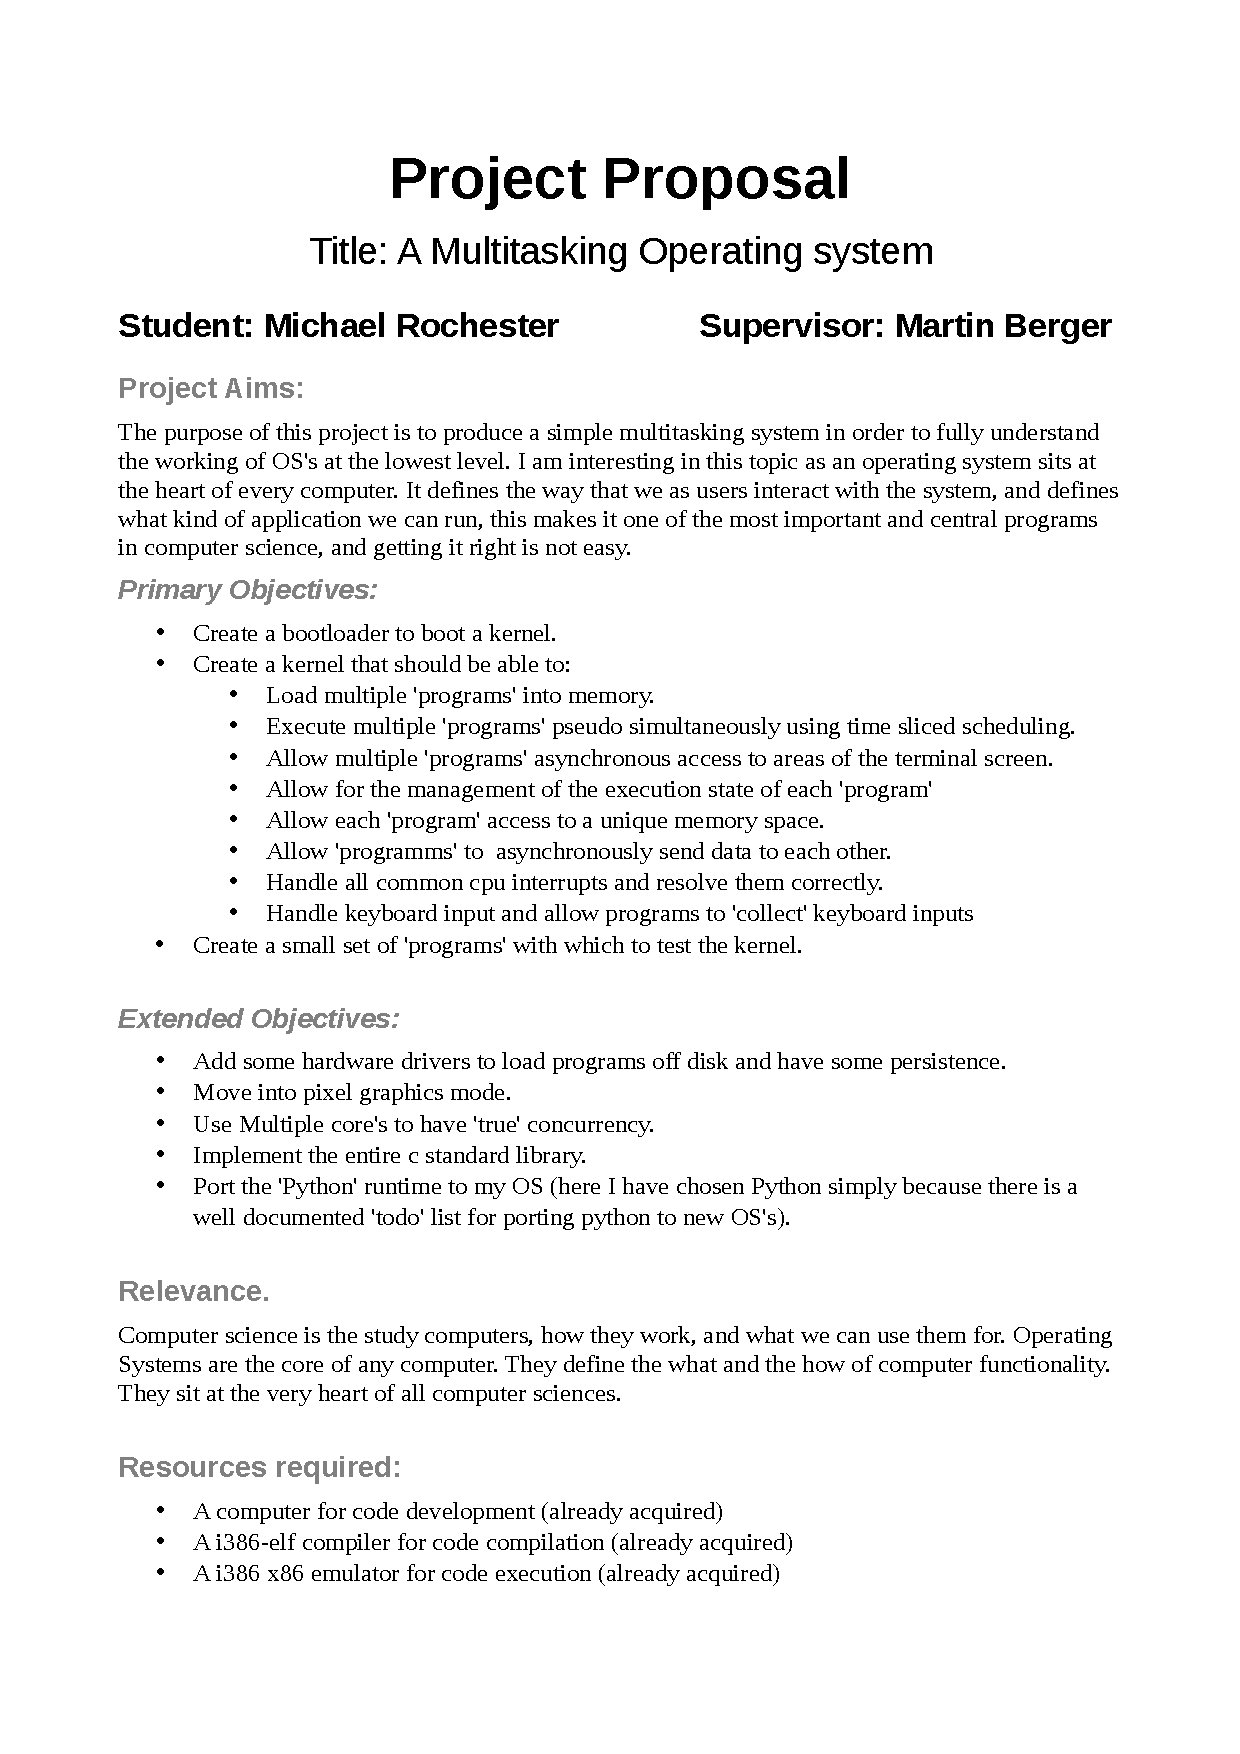
\includepdf[pages=-]{images/proposal_doc}




\bibliography{report}
\bibliographystyle{unsrt}

\end{document}